
% Question 9
\question
In Figure 2, the volume of the solid right prism $ABCDEFGH$ is $1020\text{ cm}^3$. The base $ABCD$ of the prism is a trapezium, where $AD$ is parallel to $BC$. It is given that $\angle BAD = 90^\circ$, $AB = 12\text{ cm}$, $BC = 6\text{ cm}$ and $DE = 10\text{ cm}$.

\begin{center}
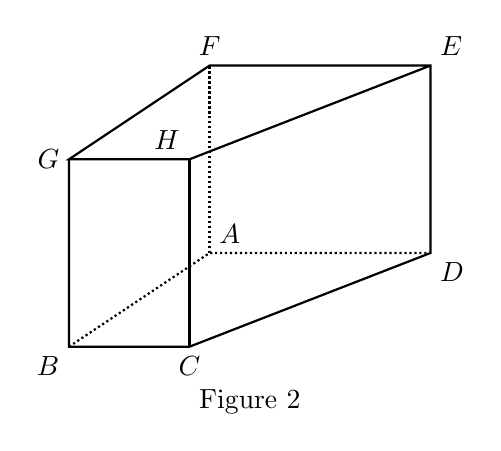
\begin{tikzpicture}[scale=0.85]
\coordinate (B) at (0,0);
\coordinate (C) at (1.8,0);
\coordinate (A) at (2.1, 1.4);
\coordinate (D) at (5.4, 1.4);
\coordinate (G) at (0, 2.8);
\coordinate (H) at (1.8, 2.8);
\coordinate (F) at (2.1, 4.2);
\coordinate (E) at (5.4, 4.2);

\draw[thick] (G) -- (B) -- (C) -- (D) -- (E) -- (F) -- (G) -- (H) -- (E);
\draw[thick] (H) -- (C);
\draw[thick, densely dotted] (B) -- (A) -- (D);
\draw[thick, densely dotted] (A) -- (F);

\node[below left] at (B) {$B$};
\node[below] at (C) {$C$};
\node[below right] at (D) {$D$};
\node[above right] at (E) {$E$};
\node[above] at (F) {$F$};
\node[left] at (G) {$G$};
\node[above left] at (H) {$H$};
\node[above right] at (A) {$A$};
\node[below=12pt] at (2.7, 0) {Figure 2};
\end{tikzpicture}
\end{center}

Find
\begin{parts}
\part the length of $AD$,
\part the total surface area of the prism $ABCDEFGH$. \\*
\null\rmarks{5}
\end{parts}

\begin{solution}
\begin{parts}
\part Let $x\text{ cm}$ be the length of $AD$.
\begin{align*}
\frac{(6 + x)(12)}{2}(10) &= 1020 \quad &\text{(1M)} \\
x &= 11 \quad &\text{(1A)}
\end{align*}
Thus, the length of $AD$ is $11\text{ cm}$.
\part 
\[
CD = \sqrt{12^2 + (11 - 6)^2} = 13\text{ cm} \quad \text{(1M)}
\]
The total surface area of the prism $ABCDEFGH$ is
\begin{align*}
&= (12 + 11 + 13 + 6)(10) + \frac{(6 + 11)(12)}{2}(2) \quad &\text{(1M)} \\
&= 624\text{ cm}^2 \quad &\text{(1A)}
\end{align*}
\end{parts}
\end{solution}


% Question 11
\question
Let $\$C$ be the cost of painting a can of surface area $A\text{ m}^2$. It is given that $C$ is the sum of two parts, one part is a constant and the other part varies as $A$. When $A = 2$, $C = 62$; when $A = 6$, $C = 74$.
\begin{parts}
\part Find the cost of painting a can of surface area $13\text{ m}^2$. \rmarks{4}
\part There is a larger can which is similar to the can described in (a). If the volume of the larger can is $8$ times that of the can described in (a), find the cost of painting the larger can. \rmarks{2}
\end{parts}

\begin{solution}
\begin{parts}
\part Let $C = r + sA$, where $r$ and $s$ are non-zero constants. \hfill (1A) \\
So, we have $r + 2s = 62$ and $r + 6s = 74$. \hfill (1M) \\
Solving, we have $r = 56$ and $s = 3$. \hfill (1A) \\
The required cost is
\[
56 + 3(13) = \$95 \quad \text{(1A)}
\]
\part Since the volume of the larger can is $8$ times that of the can described in (a), the surface area of the larger can is $4$ times that of the can described in (a). \hfill (1M) \\
The surface area of the larger can is
\[
(13)(4) = 52\text{ m}^2
\]
The required cost is
\[
56 + 3(52) = \$212 \quad \text{(1A)}
\]
\end{parts}
\end{solution}

% Question 12
\question
Figure 3(a) shows a solid metal right circular cone of base radius $48\text{ cm}$ and height $96\text{ cm}$.

\begin{center}
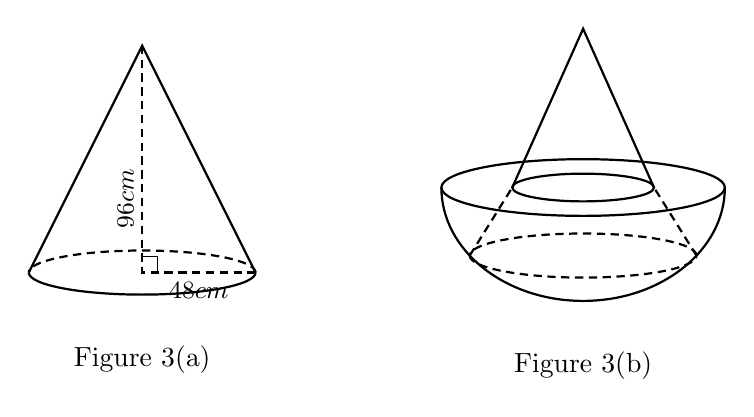
\begin{tikzpicture}[scale=0.8]
% Figure 3(a)
\begin{scope}[shift={(-3.5, 0)}]
\draw[thick] (-1.8, 0) arc (180:360:1.8cm and 0.35cm);
\draw[thick, densely dashed] (1.8, 0) arc (0:180:1.8cm and 0.35cm);
\draw[thick] (-1.8, 0) -- (0, 3.6) -- (1.8, 0);
\draw[thick, densely dashed] (0, 3.6) -- (0, 0) -- (1.8, 0);
\draw (0, 0.25) -- (0.25, 0.25) -- (0.25, 0);
\node[rotate=90, left, yshift=6pt] at (0, 1.8) {\small $96\text{ cm}$};
\node[below] at (0.9, 0) {\small $48\text{ cm}$};
\node[below=15pt] at (0, -0.35) {Figure 3(a)};
\end{scope}

% Figure 3(b)
\begin{scope}[shift={(3.5, 0)}]
% Hemisphere (radius 2.25)
\draw[thick] (0, 1.35) ellipse (2.25cm and 0.45cm);
\draw[thick] (-2.25, 1.35) arc (180:360:2.25cm and 1.8cm);
% Cone base at y = 0 (radius 1.8)
\draw[thick, densely dashed] (-1.8, 0.27) arc (180:360:1.8cm and 0.35cm);
\draw[thick, densely dashed] (1.8, 0.27) arc (0:180:1.8cm and 0.35cm);
% Cone intersection with milk surface at y = 1.35 (radius 1.125)
\draw[thick] (0, 1.35) ellipse (1.125cm and 0.22cm);
% Cone sides
\draw[thick, densely dashed] (-1.8, 0.27) -- (-1.125, 1.35);
\draw[thick, densely dashed] (1.8, 0.27) -- (1.125, 1.35);
\draw[thick] (-1.125, 1.35) -- (0, 3.87) -- (1.125, 1.35);
\node[below=15pt] at (0, -0.45) {Figure 3(b)};
\end{scope}
\end{tikzpicture}
\end{center}

\begin{parts}
\part Find the volume of the circular cone in terms of $\pi$. \rmarks{2}
\part A hemispherical vessel of radius $60\text{ cm}$ is held vertically on a horizontal surface. The vessel is fully filled with milk.
\begin{subparts}
\subpart Find the volume of the milk in the vessel in terms of $\pi$.
\subpart The circular cone is now held vertically in the vessel as shown in Figure 3(b). A craftsman claims that the volume of the milk remaining in the vessel is greater than $0.3\text{ m}^3$. Do you agree? Explain your answer. \\*
\null\rmarks{5}
\end{subparts}
\end{parts}

\begin{solution}
\begin{parts}
\part The required volume is
\begin{align*}
&= \frac{1}{3}\pi(48)^2(96) \quad &\text{(1M)} \\
&= 73728\pi\text{ cm}^3 \quad &\text{(1A)}
\end{align*}
\part
\begin{subparts}
\subpart The required volume is
\begin{align*}
&= \frac{2}{3}\pi(60)^3 \quad &\text{(1M)} \\
&= 144000\pi\text{ cm}^3 \quad &\text{(1A)}
\end{align*}
\subpart Let $h\text{ cm}$ be the height of the frustum under the surface of the milk and $r\text{ cm}$ be the base radius of the circular cone above the surface of the milk.
\begin{align*}
h &= \sqrt{60^2 - 48^2} = 36 \quad &\text{(1M)} \\
\frac{r}{48} &= \frac{96 - 36}{96} \implies r = 30
\end{align*}
The volume of the milk remaining in the vessel is
\begin{align*}
&= 144000\pi - \left(73728\pi - \frac{1}{3}\pi(30)^2(96 - 36)\right) \quad &\text{(1M)} \\
&= 88272\pi\text{ cm}^3 \\
&\approx 0.2773146667\text{ m}^3 < 0.3\text{ m}^3
\end{align*}
Thus, the claim is disagreed. \hfill (1A f.t.)
\end{subparts}
\end{parts}
\end{solution}